\documentclass{beamer}

\usepackage[english]{babel}
\usepackage[T1]{fontenc}
\usepackage{beamerthemeAntibes}
\usepackage{graphicx}
\usepackage{listings}
\usepackage[utf8]{inputenc} 
\usepackage{epsfig}  
\usepackage{amsmath} 
\usepackage{multicol}
\usepackage{amsfonts}
\usepackage{hyperref}
\usepackage{listings}
\usepackage{tkz-graph}
\usepackage{algorithm}
\usepackage{algorithmic}

\usetikzlibrary{arrows}

\newcommand{\vect}[1]{\ensuremath{\boldsymbol{#1}}}
\renewcommand{\algorithmicrequire}{\textbf{Input:}}
\renewcommand{\algorithmicensure}{\textbf{Output:}}

\title{Social Network Project}
\author{Francesco Siani, Marco Mecchia}
\institute{Università degli Studi di Salerno}


\begin{document}
\SetVertexNormal[Shape      = circle,
                 FillColor  = orange,
                 LineWidth  = 2pt]
\SetUpEdge[lw         = 1.5pt,
           color      = black,
           labelcolor = white,
           labeltext  = red,
           labelstyle = {sloped,draw,text=blue}]

\section{Introduction}
\begin{frame}
   \maketitle
\end{frame}

\begin{frame}
\frametitle{Overview}
\small
\tableofcontents
\end{frame}

\begin{frame}
\frametitle{Introduction}
The purpose of our work is to test different algorithms in the three fundamental areas for assembling any search engine offering a Sponsored Search system:
\begin{description}
\item[Ranking]  of web documents
\item[Matching] of words inside documents
\item[Auctions] for acquiring advertisement slots.
\end{description}
\end{frame}

\section{Ranking}

\subsection{Page Rank}
\begin{frame}
\frametitle{Web Model}
For our porpuses, we model the web as a graph $G = (V,E)$, where:
\begin{itemize}
\item $V$ is the set of web pages.
\item $E$ are the hyperlinks connecting the pages.
\end{itemize}
\vfill
The graph is directed since hyperlinks are unidirectional.
\end{frame}

\begin{frame}
\frametitle{Web Transition Matrix}
Graph can be easily rappresented as matrices. 
\vfill
One rappresentation is the \emph{Transition Matrix}:
\[ T(p,q) =
\begin{cases}
	0       & \quad \text{if } (q,p) \notin E\\
	1/\omega(q)  & \quad \text{if } (q,p) \in E\\
\end{cases}
\]
\vfill
Where $\omega(q)$ is the outdegree of node $q$.
\end{frame}

\begin{frame}
\frametitle{PageRank}
PageRank is a well known algorithm that uses link information to assign global importance scores to all pages on the web. 
\begin{itemize}
\item The intuition behind PageRank is that a webpage is important if several other pages point to it.
\item PageRank is based on \emph{Mutual Reinforcement} between pages.
\end{itemize}
\vfill
The PageRank score $r(p)$ of a page $p$ is defined as:
$$ r(p) = \alpha \cdot \displaystyle\sum_{q:(q,p) \in E} \frac{r(q)}{\omega(q)} + (1 - \alpha) \cdot \frac{1}{n} $$
\end{frame}

\begin{frame}
\frametitle{Generalized Pagerank}
Given the transition matrix of a graph $T$, PageRank can be easily generalized in a matricial form.
$$\vect{r} = \alpha \cdot \vect{T} \cdot r + (1 - \alpha) \cdot \vect{d}$$
Where $\vect{d}$ is a \emph{static score distribution vector} of arbitrary, non-negative entries summing up to one.
\end{frame}

\subsection{Trust Rank and Spammass}
\begin{frame}
\frametitle{Topic-Sensitive Pagerank}
\begin{itemize}
\item Since its introduction, a great number of improvements have been tought for PageRank.
\item One of the main ideas is to use more than one vector of PageRank based on the \alert{topic} in which the user is interested.
\item In fact, one can use the \emph{static score distribution vector} seen in previous slide and the initial ranks to weight some pages more than others.
\item Motivations: different people have different interests, biased random walks.
\end{itemize}
\end{frame}

\begin{frame}
\frametitle{The spam farm problem}
One of the main ideas to fool pagerank is the \alert{spam farm}, which is made up by:
\vfill
\begin{itemize}
\item A target page whose contents are likely to be matched by the search engine.
\item A \alert{big} set of spam pages whose contents are uninfluent, but they are two-ways linked to the target page.
\end{itemize}
\vfill
With such architecture, PageRank gives the target page a very high score.
\end{frame}

\begin{frame}
\frametitle{An example of spam farm}
\begin{tikzpicture}
\Vertex[x=0 ,y=1]{b}
\Vertex[x=0 ,y=2]{c}
\Vertex[x=0 ,y=3]{d}
\Vertex[x=0 ,y=4]{e}
\Vertex[x=0 ,y=5]{f}
\Vertex[x=0 ,y=6]{g}
\Vertex[x=0 ,y=7]{h}
\Vertex[x=8 ,y=7]{r}
\Vertex[x=2 ,y=7]{s}
\Vertex[x=3 ,y=7]{t}
\Vertex[x=4 ,y=7]{u}
\Vertex[x=5 ,y=7]{a2}
\Vertex[x=6 ,y=7]{z}
\Vertex[x=7 ,y=7]{a}
\Vertex[x=10 ,y=1]{i}
\Vertex[x=10 ,y=2]{l}
\Vertex[x=10 ,y=3]{m}
\Vertex[x=10 ,y=4]{n}
\Vertex[x=10 ,y=5]{o}
\Vertex[x=10 ,y=6]{p}
\Vertex[x=10 ,y=7]{q}
\Vertex[x=8 ,y=1]{a1}
\Vertex[x=2 ,y=1]{x}
\Vertex[x=3 ,y=1]{v}
\Vertex[x=4 ,y=1]{y}
\Vertex[x=5 ,y=1]{j}
\Vertex[x=6 ,y=1]{k}
\Vertex[x=7 ,y=1]{w}
\Vertex[x=5 ,y=4]{target}
\tikzset{EdgeStyle/.style={<->}}
\Edge(b)(target)
\Edge(c)(target)
\Edge(d)(target)
\Edge(e)(target)
\Edge(f)(target)
\Edge(g)(target)
\Edge(h)(target)
\Edge(i)(target)
\Edge(l)(target)
\Edge(m)(target)
\Edge(n)(target)
\Edge(o)(target)
\Edge(p)(target)
\Edge(q)(target)
\Edge(a1)(target)
\Edge(a)(target)
\Edge(r)(target)
\Edge(z)(target)
\Edge(u)(target)
\Edge(s)(target)
\Edge(t)(target)
\Edge(x)(target)
\Edge(y)(target)
\Edge(j)(target)
\Edge(k)(target)
\Edge(w)(target)
\Edge(v)(target)
\Edge(a2)(target)
\end{tikzpicture}
\end{frame}

\begin{frame}
\frametitle{TrustRank: Overview}
TrustRank is a particular form of topic-sensitive Pagerank.
\vfill
\begin{itemize}
\item In this case the topic is a set of pages believed to be \alert{trustworthy}.
\item Useful to combat spam farms.
\end{itemize}
\vfill
Intuition: is very unlikely that trusted pages point to spam.
\end{frame}

\begin{frame}
\frametitle{TrustRank: Algorithm}
\begin{algorithm}[H]
\small
\begin{algorithmic}[1]
\REQUIRE $\vect{T}, N, L, \alpha_\beta, M_B$
\ENSURE $\vect{t^*}$
\STATE{$\vect{s}$ = SelectSeed(...)}
\STATE{$\vect{\sigma}$ = Rank($\{1 \dots N \}$, $\vect{s}$)}
\STATE{$\vect{d} = \vect{0}_N$}
\FOR{$i=1$ to $L$}
\IF{$O(\sigma(i)) == 1$} 
\STATE{$\vect{d}(\sigma(i)) = 1$}
\ENDIF
\ENDFOR
\STATE{$\vect{d} = \vect{d}/|\vect{d}|$}
\STATE{$\vect{t^*} = \vect{d}$}
\FOR{$i=1$ to $M_B$}
\STATE{$\vect{t^*} = \alpha_\beta \cdot \vect{T} \cdot \vect{t^*} + (1-\alpha_b) \cdot \vect{d}$}
\ENDFOR
\end{algorithmic}
\caption{TrustRank}
\label{alg:seq}
\end{algorithm}
\end{frame}

\begin{frame}
\frametitle{Methods to selects seeds}
There are two main ways to implement the function SelectSeed which returns the set $\vect{s}$ on which invoke the oracle:
\vfill
\begin{enumerate}
\item Nodes with high pagerank score.

In this way, if the target of a spam farm has a high pagerank is judged by the oracle.
\item Nodes with high inverse pagerank score.

In this way, we use the oracle on nodes that have a lot of outgoing links.
\end{enumerate}
\vfill
Our implementation uses a hybrid tecnicque.
\end{frame}

\begin{frame}
\frametitle{SpamMass}
SpamMass is a useful tecnique to identify probably spam pages.

\begin{itemize}
\item It is based both on PageRanks and TrustRanks.
\item Once the probably spam nodes are identified, they can be ignored by the search engine.
\end{itemize}
Given $t_r$ and $p_r$ the TrustRank and PageRank of the page $r$, the SpamMass $s_r$ is given by:
$$s_r = \frac{p_r - t_r}{p_r}$$
\end{frame}

\section{Matching}
\subsection{Best Match}
\begin{frame}
\frametitle{The idea of Best Match}
Given a query $q$, containing $n$ query words, and a set of documents $S$, we define Best Match as a method that finds a subset of document $S'$ such that:
\begin{itemize}
\item each document $s_i$ of $S'$ has a "reasonable" number of query words in it
\end{itemize}
\medskip
According to this definition the basic Best Match consists of:
\begin{itemize}
\item counting how many query words documents have
\begin{itemize}
\item we call this value "score" of a document
\item it is at maximum $n$
\end{itemize}
\item ordering in decreasing order of score the documents (optional)
\item return all documents whose score is "reasonable"
\begin{itemize}
\item we use a threshold to define what is "reasonable"
\end{itemize}
\end{itemize}
\end{frame}

\begin{frame}
\frametitle{Refining the Best Match}
Two are the basic refinements to have a more efficient Best Match algorithm:
\begin{enumerate}
\item Use an inverted index.
\begin{itemize}
\item in the form (word -> list of documents containing the word).
\item the keys of the dataset are the query words.
\item we can have in O(1) all the documents containing a determined word.
\end{itemize}
\item Use the frequency of the word in a document instead of assigning score 1. 
\begin{itemize}
\item defined as number of occurrences in document $d$ / length($d$).
\item it represents the \emph{relevance} of a word in a particular document.
\end{itemize}	
\end{enumerate}
The main drawbacks of this refinements are the need of precomputation and special data structures.
\end{frame}

\subsection{Improved Best Match}
\newcounter{sauvegardeenumi}
\newcommand{\asuivre}{\setcounter{sauvegardeenumi}{\theenumi}}
\newcommand{\suite}{\setcounter{enumi}{\thesauvegardeenumi}}

\begin{frame}
\frametitle{Improved Best Match}
We implemented also the following improved version of Best Match:
\begin{enumerate}
\item Sort offline documents in each inverted index in order of frequency of the term at which the inverted index refers.
\item For every query term define its possible impact on the score as the frequency of the most frequent document in its index
\item Sort the query terms in decreasing order of impact.
\item Consider the first 20 documents in the index of the first query term (if the first query term has an index with less than 20 documents, then complete with the first documents in the index of the next query term).
\asuivre
\end{enumerate}
\end{frame}

\begin{frame}
\frametitle{Improved Best Match}
\begin{enumerate}	
\suite
\item Compute the score for each of these documents.
\item Consider the first term in which there are documents that have not been scored.
\item Consider the first non-scored document in the index of this term.
\item If the frequency of the current term in the current document plus the sum of the impact of next terms is larger than the score of the 20-th scored document, then score this document and repeat from 7, otherwise consider the next.
\end{enumerate}
\end{frame}

\section{Experiments}
\subsection{Dataset}
\begin{frame}
\frametitle{Creating the Dataset}
Our experiments ran on a set of approximatively 30000 pages created this way:
\begin{itemize}
\item We choosed a web-page for each of the 15 categories listed in https://www.dmoz.org/
\item For every of these web pages we crawled 2000 pages by using the Wibbi online crawler
\item Once generated the graph, from each pair of sets of 2000 pages, we choosed at random 10 pairs of vertices (u, v) with u being a page in the first set and v being a page in the second set and we added a link from u to v (if this link was absent).
\end{itemize}
\end{frame}

\begin{frame}
\frametitle{Creating the Dataset}
Here is the complete list of the websites chosen.
\begin{table}[]
	\centering
	\resizebox{\textwidth}{!}{%
		\begin{tabular}{lll}
			\textbf{Category} & \textbf{Website}       & \textbf{Description}                                                                                                                                                                                         \\
			Arts              & www.imdb.com           & The Internet Movie Database \\
			Business          & www.moodys.com         & Corporate finance, banking                                                                                                                        \\
			Computers         & www.ibm.com            &International Business Machines Corporation.                                                                                                                                                     \\
			Games             & www.ign.com            & Videogame news     \\
			Health            & www.who.int            & World Health Organization \\
			Home              & www.allrecipies.com          & Recipe search  \\
			Kids              & www.cartoonnetwork.com & The home of cartoons online
		\end{tabular}%
	}
\end{table}
\end{frame}

\begin{frame}
\frametitle{Creating the Dataset}
\begin{table}[]
	\centering
	\resizebox{\textwidth}{!}{%
		\begin{tabular}{lll}
			\textbf{Category} & \textbf{Website}       & \textbf{Description}                                                                                                                                                                                       \\
			News              & www.foxnews.com        & Breaking News\\
			Recreation        & www.lego.com           & Producer of bilding blocks.                                                                                                                                                                             \\
			Reference         & www.stackoverflow.com     & Q \&\, A site for computer science topics.\\
			Science           & www.researchgate.net           & Researchgate is a network dedicated to science and research.                    \\
			Shopping          & www.ebay.com         & One of the most known shopping website\\
			Sports            & www.nba.com            & The official site of the National Basketball Association\\
			Regional          & www.lonelyplanet.com   & Offers travel advice, detailed maps, travel news                                                   
		\end{tabular}%
	}
\end{table}
\end{frame}

\begin{frame}
\frametitle{Adding the spam farm}
To test the utility of SpamMass, we added to our dataset a spam farm in the following way:
\vfill
\begin{enumerate}
\item We created a target page and 100 supporting pages.
\item The target page contains the 500 words with the smaller index among the one contained in the above 30000 nodes.
\item We created 30 random links from the original 30000 nodes to the target pages.
\end{enumerate}
\end{frame}

\subsection{PageRanks and SpamMass results}

\begin{frame}
\frametitle{PageRank distribution(Plot)}
     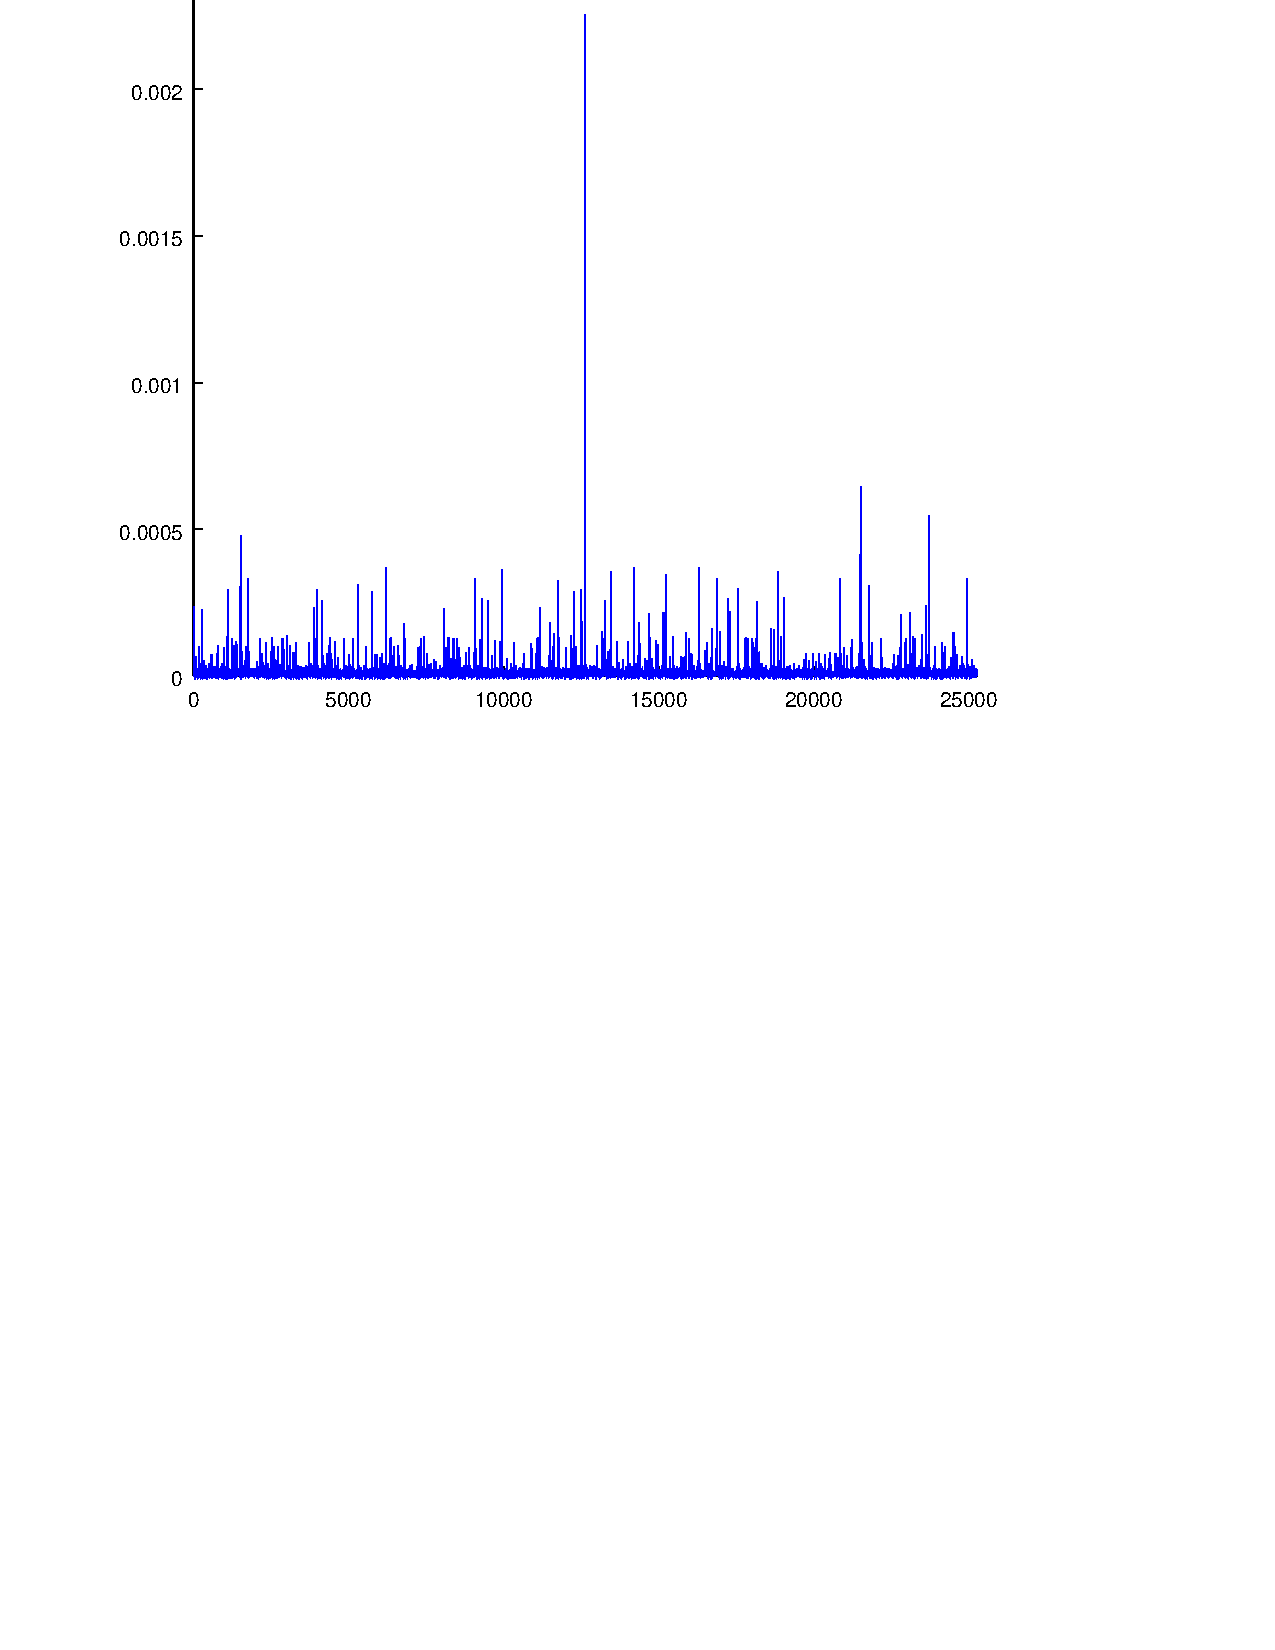
\includegraphics[width=\textwidth,keepaspectratio]{Pictures/Pagerank.pdf}
\end{frame}

\begin{frame}
\frametitle{PageRank performance}
PageRank performed quite well on our dataset.
\begin{itemize}
\item Even with small confidence values, its convergence took never more than 100 steps.
\item Sorting the scores in descending way we found most of the sites from which we started the crawling, or pages related to them, to have top scores.
\item Unfortunately, the top score was achieved by the 'target' page of the spam farm.
\end{itemize}
\end{frame}

\begin{frame}
\frametitle{SpamMass}
Our analysis was slightly different for what's concering SpamMass. 
\begin{itemize}
\item SpamMass scores depend on TrustRanks, which depend on the trusted pages given to the algorithm.
\item We noticed that when the trusted pages were few a lot of pages got TrustRank 0, so were considered spam by SpamMass.
\item So we increased the size of the trusted pages vector each time of 10 pages and calculated SpamMass with the different TrustRanks.
\item Each time we took five pages from the set of pages with highest PageRanks and five from the set of pages with highest \emph{inverted} PageRanks.
\end{itemize}
\end{frame}

\begin{frame}
\frametitle{SpamMass performance}
We proceded raising the oracled pages as indicated above by but the trend remained...
\begin{itemize}
\item With 80 pages oracled and given to TrustRank, with a SpamMass threshold of 0.95, still \alert{$35\%$} of the pages are considered spam!!!
\item Boosting the number of trusted pages to 2000 and with a threshold of $0.99$ only the $7\%$ of nodes were considered spam.
\end{itemize}
\vfill
The target page of the spam was always marked as spam.
\end{frame}

\begin{frame}
\frametitle{SpamMass - Conclusions}
SpamMass is useful for identify probable spam pages, but it must be used cautiosly since it relies on TrustRank.
\begin{itemize}
\item If there are too few trusted pages, a lot of pages could be exchaged for spam, even the good ones.
\item On the other hand, if there are too many trusted pages, TrustRanks tend to PageRanks, thus not identifing correctly spam pages.
\item Moreover, if a lot of pages must be judged by the oracle function, we need an automatic oracle, since an human would only be time consuming.
\end{itemize}
\end{frame}

\subsection{Matching algorithms results}
\begin{frame}
\frametitle{Experiment configuration}
For the comparison between the two matching algorithms we set up the following configuration:
\begin{itemize}
\item For each query length $l$.
\item Generate a random query of length $l$ and use both the algorithms to match the query, keeping track of results and execution time.
\end{itemize}

The two algorithms returned \alert{always} the same results so we focused on the execution time.
\end{frame}

\begin{frame}
	\frametitle{Time comparison BestMatch vs ImprovedBestMatch}
	\begin{center}
	%\includegraphics[scale=0.32]{img/Matching/Tempi.PNG} 
	\end{center}
\end{frame}

\section{Conclusions}
\begin{frame}
\centering 
\Huge{Thank you for the attention.}
\end{frame}

\end{document}